\graphicspath{{./figures}}

\section{High-Level System}
A complete high-level system block diagram illustrating the system-level decisions is shown in Figure \ref{fig:complete_system}. Note that the yellow blocks are external (i.e. assumed to be available already).

\begin{figure}[!htb]
    \centering
    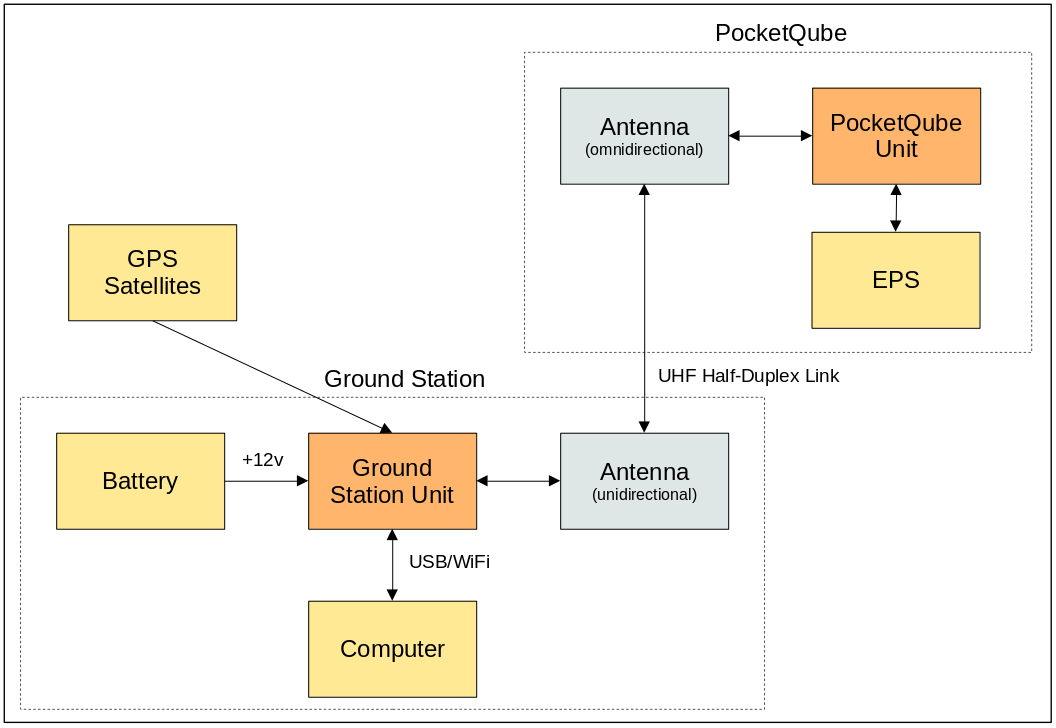
\includegraphics[width=0.8\textwidth]{complete_system.png}
    \caption{High-Level System Diagram}
    \label{fig:complete_system}
  \end{figure}

\newpage
\subsection{Methodology}
Since a large number of sub-systems are required on the ground-station, either IC \textit{modules} or simple \textit{reference designs} will be form the basic building blocks of the system. Only if no modules or designs are found to meet the system requirements, will a more custom solution be developed. The ground station will be powered via +12V from a nearby vehicle, and the PocketQube will be powered from an on-board EPS (another PQ unit). Both sub-systems should be designed such that testing without a vehicle/EPS is also possible.

\subsection{Tracking}
It is assumed that open-loop path-predicted tracking is generally adequate for high-altitude balloons, given the number of tools available to predict their flight path. In this sense, the ground station requires at least a GPS connection, as well as a means of determining true north (such as a magnetometer) for beem steering. The path data will be uploaded to the ground station via USB from a system computer. If time allows, direct GPS tracking will be added as a method of "closing the loop", and to improve pointing accuracy.

\subsection{Custom Link}
Half-duplex communication will be designed for, since full-duplex is assumed to be unnecessary for this type of link. This is due to the nature of the link itself (i.e. downlink telemetry), as well as the simple command-response ("telecommand") pattern that would be used for bi-directional communication. For the given flight path, a goal of at least 9600 downlink baud rate will be designed for at the approximate 120 km range. LoRa will be explored as the main modulation technique, however a secondary scheme such as GFSK should be considered as a backup, which is well-established and is still suitable over such a range. The 433 MHz amateur band (430 to 440 MHz) will be utilized.